
The optimizing compiler is critically important for achieving high performance. Just try running a program compiled with no optimization at all to appreciate the role of the compiler: it is not uncommon for an unoptimized program (optimization level zero) to run an order of magnitude slower than the program compiled with all optimizations enabled.

Very often, however, it is the case that the optimizer can use some help from the programmer. This help can take the form of very subtle and often counter-intuitive changes. Before we look at some specific techniques to improve the optimization of your code, it helps to understand how the compiler sees your program.

\subsubsubsection{10.2.1\hspace{0.2cm}Basics of compiler optimizations}

The most important thing you must understand about optimization is that any code that is correct must remain correct. Correct here has nothing to do with your view of what is correct: the program may have bugs and give an answer you consider wrong, but the compiler must preserve this answer. The only exception is a program that is ill-defined or invokes undefined behavior: if the program is incorrect in the eyes of the Standard, the compiler is free to do whatever it wants. We will examine the implications of this in the next chapter. For now, we are going to assume that the program is well defined and uses only valid C++. The compiler, of course, is restricted in what changes it can make by the requirement that the answers must not change for any combination of inputs. The latter is very important: you may know that a certain input value is always positive or a certain string is never more than 16 characters long, but the compiler does not know that (unless you find a way to tell it). The compiler can only make the optimizing transformation if it can be proven that this transformation results in a perfectly equivalent program: a program that produces the same outputs for any inputs. In practice, the compiler is also limited in how complex of a proof it can manage before it gives up.

This understanding that it's not what you know, it's what you can prove is the key to successfully interacting with the compiler through code to achieve better optimizations. Basically, the rest of this chapter shows different ways in which you can make it easier to prove that certain desirable optimizations do not alter the result of the program.

A compiler is also restricted with regard to what information it has about the program. It has to work with only what is known at compile-time, has no knowledge of any runtime data, and has to assume that any legal state is possible at runtime.

Here is a simple example that illustrates this. First, consider this code:

\begin{lstlisting}[style=styleCXX]
std::vector<int> v;
… fill v with data … 
for (int& x : v) ++x;
\end{lstlisting}

The focus of our attention is the last line, the loop. The performance may be better if the loop is manually unrolled: as written, there is one branch (loop termination condition) for every increment. Unrolling the loop reduces this overhead. In a simple case of a vector with, say, only two elements, it is even better to remove the loop completely and just increment both elements. However, the size of the vector is an example of runtime information. The compiler may be able to generate a partially unrolled loop with some extra branches to handle all possible vector sizes, but it cannot optimize the code for a  particular size.

Contrast it with this code:

\begin{lstlisting}[style=styleCXX]
int v[16];
… fill v with data … 
for (int& x : v) ++x;
\end{lstlisting}

Now the compiler knows exactly how many integers are processed in the loop. It can unroll the loop and even replace single integer increments with vector instructions that operate on several numbers at once (AVX2 instruction set on x86, for example, can add 8 integers at once). 

What if you know that the vector always has 16 elements? Probably does not matter. What matters is whether the compiler knows this and can prove it with certainty. This is harder than you think. For example, consider this code:

\begin{lstlisting}[style=styleCXX]
constexpr size_t N = 16;
std::vector<int> v(N);
… fill v with data … 
for (int& x : v) ++x;
\end{lstlisting}

The programmer went out of their way to make it obvious that the vector size is a compile-time constant. Is the compiler going to optimize the loop? Possibly. It all depends on whether the compiler can prove that the vector size does not change. How would it change? Ask yourself, what could be hiding in the code that fills the vector? Not what you know to be there, but what can be learned from the code itself? If all the code is written between the two lines, the construction and the increment loop, the compiler can, in theory, know everything (in practice, the compiler will give up if this code fragment is too long and assume that anything is possible otherwise compilation times will explode). But if you call a function and that function has access to the vector object, the compiler has no way of knowing whether that function changes the size of the vector unless the function is inlined. A helpful function name like fill\_vector\_without\_resizing() is only helpful to the programmer. 

Even if there are no function calls that take v as an argument, we are still not in the clear. How else might the function get access to the vector object? If the vector v is a local  variable declared in a function scope, it probably cannot. But if v is a global variable, then  any function can have access to it. Similarly, if v is a class member variable, any member  function or friend function can have access to it. So, if we call a non-inlined function that  does not get direct access to v through its argument list, it may still be able to access v through other means (and the less is said about the truly evil practice of creating global pointers to local variables, the better). 

From the programmer's point of view, it is easy to overestimate the knowledge the compiler has, based on the knowledge the programmer has about what is really going on in the program. Also, remember that puzzling things out is not one of the compiler's strengths, most of the time. For example, you can add an assert just before the loop:

\begin{lstlisting}[style=styleCXX]
constexpr size_t N = 16;
std::vector<int> v(N);
… fill v with data … 
assert(v.size() == N); // if (v.size() != N) abort();
for (int& x : v) ++x;
\end{lstlisting}

Some compilers, at the highest optimization level and in simple contexts, will deduce that the execution flow cannot get to the loop unless the vector has exactly 16 elements and will optimize for that size. Most will not. By the way, we are assuming that the asserts are enabled (NDEBUG is undefined), or you use your own assert.

The basic example we have considered already has the key elements of the techniques used to assist the compiler with optimizing the code:

\begin{itemize}
\item
Non-inlined functions disrupt most optimizations because the compiler has to assume that a function whose code it does not see can do anything it is legally allowed to do. 

\item
Global and shared variables are terrible for optimization

\item
The compiler is more likely to optimize a short and simple code fragment than a long and complex one.
	
\end{itemize}

The first and the last notions are somewhat in conflict with each other. Most optimizations in the compilers are limited to what's known as basic blocks of code: these are blocks with only one entry point and only one exit point. They serve as nodes in the flow control graph of a program. The reason basic blocks are important is that the compiler can see everything that is going on inside the block, so it can reason about code transformations that do not change the output. The advantage of inlining is that it increases the size of the basic blocks. The compiler does not know what a non-inlined function does, so it has to assume the worst. But if the function is inlined, the compiler knows exactly what it's doing (and, more importantly, what it's not doing). The disadvantage of inlining is also that it increases the size of the basic blocks: the compiler can analyze only so much code without making compilation time unreasonable. Inlining is really important for compiler optimizations for reasons we are going to explore now.


\subsubsubsection{10.2.2\hspace{0.2cm}Function inlining}

Inlining is done by the compiler when it replaces a function call with a copy of the body of the function. In order for this to happen, the inlining must be possible: the definition of the function must be visible during the compilation of the calling code, and the function that is being called must be known at compile time. The first requirement is relaxed in some compilers that do whole-program optimizations (still uncommon). The second requirement rules out virtual function calls and indirect calls through function pointers. Not every function that can be inlined ends up inlined: the compiler has to weigh the code bloat against the benefits of inlining. Different compilers have different heuristics for inlining. The inline keyword of C++ is only a suggestion, and the compiler can disregard it.

The most obvious benefit of function call inlining is that it eliminates the cost of the function call itself. This is also the least important benefit in most cases: the function calls are not that expensive. The main benefit is that the compiler is very limited in what optimizations it can do across the function calls. Consider this simple example:

\begin{lstlisting}[style=styleCXX]
double f(int& i, double x) {
	double res = g(x);
	++i;
	res += h(x);
	res += g(x);
	++i;
	res += h(x);
	return res;
}
\end{lstlisting}

Is the following a valid optimization?

\begin{lstlisting}[style=styleCXX]
double f(int& i, double x) {
	i += 2;
	return 2*(g(x) + h(x));
}
\end{lstlisting}

If you answered yes, you are still looking at this through the programmer's eyes instead of the compiler's eyes. There are so many ways in which this optimization can break the code (none of which are probably true for any reasonable program you would write, but the one assumption the compiler cannot make is that of a reasonable programmer). 

\begin{itemize}
\item
First, the functions g() and h() can produce output, in which case eliminating the repeated function calls would change the observable behavior. 

\item
Second, a call to g() might lock some mutex, and the call to h() might unlock it, in which case the order of execution – call g() to lock, increment i, call h() to unlock – is really important. 

\item
Third, the results of g() and h() may be different even with the same arguments: they could, for example, use random numbers inside. 

\item
Finally (and this possibility is most often missed by programmers), the variable i is passed by reference, so we don't know what else the caller might have done with it: it could be a global variable, or some object might store a reference to it, s, one way or another, the functions g() and h() might operate on i even though we don't see it being passed into these functions. 
	
\end{itemize}

On the other hand, if the functions g() and h() are inlined, the compiler can see exactly what is going on, for example:

\begin{lstlisting}[style=styleCXX]
double f(int& i, double x) {
	double res = x + 1; // g(x);
	++i;
	res += x – 1; // h(x);
	res += x + 1; // g(x)
	++i;
	res += x – 1; // h(x);
	return res;
}
\end{lstlisting}

The entire function f() is now one basic block, and the compiler has only one restriction: preserve the returned value. This is a valid optimization:

\begin{lstlisting}[style=styleCXX]
double f(int& i, double x) {
	i += 2;
	return 4*x;
}
\end{lstlisting}

The effect of the inlining on the optimization can trickle down quite far. Consider the destructor of an STL container, say, std::vector<T>. One of the steps it must do is to invoke the destructors on all objects in the container:

\begin{lstlisting}[style=styleCXX]
for (auto it = crbegin(); it != crend(); ++it) it->~T();
\end{lstlisting}

The execution time of the destructor is, therefore, proportional to the size N of the vector. Unless it isn't: consider a vector of integers, std::vector<int>. The compiler knows very well what the destructor does in this case: absolutely nothing. The compiler can also see that the calls to crbegin() and crend() do not modify the vector (if you are concerned about destroying an object through a const\_iterator, think how const objects are destroyed). This entire loop, therefore, can be eliminated.

Now consider using a vector of simple aggregates:

\begin{lstlisting}[style=styleCXX]
struct S {
	long a;
	double x;
};
std::vector<S> v;
\end{lstlisting}

This time, the type T has a destructor, and again the compiler knows what it does (the compiler did generate it, after all). Again, the destructor does nothing, and the entire destruction loop is eliminated. The same goes for a default destructor:


\begin{lstlisting}[style=styleCXX]
struct S {
	long a;
	double x;
	~S() = default;
};
\end{lstlisting}

The compiler should be able to do the same optimization for an empty destructor, but only if it's inlined:

\begin{lstlisting}[style=styleCXX]
struct S {
	long a;
	double x;
	~S() {}     // Probably optimized away
};
\end{lstlisting}

On the other hand, if the class declaration only declares the destructor like the following:

\begin{lstlisting}[style=styleCXX]
struct S {
	long a;
	double x;
	~S();
};
\end{lstlisting}

and the definition is provided in a separate compilation unit, then the compiler has to generate a function call for each vector element. The function still does nothing, but it still takes time to run the loop and do N function calls. Inlining allows the compiler to optimize this time to nothing, zero.

This is the key to inlining and its effect on optimization: inlining allows the compiler to see what is not happening inside the otherwise mysterious function. Inlining has another important role: it creates a unique clone of the inlined function's body that can be optimized with the specific inputs as given by the caller. Within this unique clone, some optimization-friendly conditions may be observed that are not true in general for this function. Again, here is an example:


\begin{lstlisting}[style=styleCXX]
bool pred(int i) { return i == 0; }
… 
std::vector<int> v = … fill vector with data …;
auto it = std::find_if(v.begin(), v.end(), pred);
\end{lstlisting}

Assuming the definition of the function pred() is in the same compilation unit as the call to std::find\_if(), will the call to pred() be inlined? The answer is maybe, and it critically depends on whether or not the call to find\_if() is inlined first. Now, find\_if() is a template, so the compiler always sees the function definition. It may decide not to inline the function, regardless. If find\_if() is not inlined, then we have a function generated from the template for the specific types. Within this function, the type of the third argument is known: it's bool (*)(int), a pointer to a function that takes an int and returns a bool. But the value of this pointer is not known at compile time: the same find\_if() function can be called with many different predicates, so none of them can be inlined. Only if the compiler generates a unique clone of find\_if() for this particular call can the predicate function be inlined. Compilers will sometimes do just that; it is called, unsurprisingly, cloning. Most of the time, however, the only way to inline the predicate, or any other inner function that is passed in as a parameter, is to inline the outer function first. 

This particular example produces different results on different compilers: for example, GCC will inline both find\_if() and pred() at the highest optimization setting only. Other compilers won't do it even then. However, there is another way to encourage the compiler to inline a function call, and it does seem counter-intuitive because it adds more code to the program and makes the chain of nested function calls longer:

\begin{lstlisting}[style=styleCXX]
bool pred(int i) { return i == 0; }
… 
std::vector<int> v = … fill vector with data …;
auto it = std::find_if(v.begin(), v.end(), 
  [&](int i) { return pred(i); });
\end{lstlisting}

The paradox here is that we have added an extra layer of indirection, a lambda expression, around the same indirect function call (by the way, we assume that there is a reason the programmer does not want to simply duplicate the body of the predicate directly into the lambda). This call to pred() is actually much easier to inline, even if the compiler does not inline the find\_if() function. The reason is that this time, the type of the predicate is unique: every lambda expression has a unique type, so there is only one instantiation of the find\_if() template for these particular type parameters. The compiler is more likely to inline a function that is called only once: after all, doing so does not generate any more code. But even if the call to find\_if() is not inlined, within that function, there is only one possible value of the third argument, this value is known at compile time to be pred() and, therefore, the call to pred() can be inlined.

As an aside, we can finally clarify the answers to the question we asked all the way back in Chapter 1, Introduction to Performance and Concurrency: what is the cost of a virtual function call? First of all, the compiler typically implements a virtual call using a table of function pointers, so the call itself involves an extra layer of indirection: the CPU has to read one more pointer and do one more jump compared to a non-virtual call. This adds several more instructions to the function call, making the code of the function call about twice as expensive (with a large variation depending on the hardware and cache state). However, we usually call a function to have some work done, so the machinery of the function call is only a part of the total function execution time. Even for simple functions, it is rare to have the virtual function cost more than 10-15\% of the non-virtual one.

However, before we spend too much time counting instructions, we should question the validity of the original question: if a non-virtual function call is sufficient, that is, if we know at compile time which function will be called, why would we use a virtual function in the first place? Conversely, if we find out which function to call only at runtime, then a non-virtual function cannot be used at all, so its speed is irrelevant. Following this logic, we should compare a virtual function call against a functionally equivalent runtime solution: conditionally call one of several functions using some runtime information to choose. Using an if-else or a switch statement usually results in slower execution, at least if there are more than two versions of the function to call. The most efficient implementation is a table of function pointers, which is precisely what the compiler does with virtual functions. 

Of course, the original question was not, in truth, entirely meaningless: what if we have a polymorphic class with a virtual function but, in some cases, we know the actual type at compile time? In this case, comparing a virtual function call with a non-virtual one makes sense. We should also mention an interesting compiler optimization that applies: if the compiler can figure out the real type of the object at compile time and, thus, knows which override of the virtual function will be called, it will convert the call to non-virtual in what is known as devirtualization.

Why, though, is this discussion taking place in a section dedicated to inlining? Because we are missing the elephant in the room: the greatest impact of virtual functions on performance is that (unless the compiler can devirtualize the call) they cannot be inlined. A simple function such as int f() { return x; } results in one or even zero instructions after inlining, but the non-inlined version has the regular function call machinery, which is orders of magnitude slower. Now add the fact that without inlining, the compiler cannot know what's going on inside the virtual function and has to make the worst assumptions about every externally accessible piece of data, and you can see how, in the worst-case scenario, a virtual function call can be thousands of times more expensive.

Both effects of inlining, exposing the content of the functions, and creating a unique, specialized copy of the function, help the optimizer because they increase the amount of knowledge the compiler has about the code. As we already mentioned, it is very important to understand what the compiler really knows if you want to help it do a better job of optimizing your code. 

We will now explore different restrictions the compiler operates under, so you can develop an eye for recognizing the false constraints: something you know to be true but the compiler does not. 

\subsubsubsection{10.2.3\hspace{0.2cm}What does the compiler really know?}

Perhaps the greatest constraint on the optimization is the knowledge of what can change during the execution of this code. Why is this important? Again, here is an example:

\begin{lstlisting}[style=styleCXX]
int g(int a);
int f(const std::vector<int>& v, bool b) {
	int sum = 0;
	for (int a : v) {
		if (b) sum += g(a);
	}
	return sum;
} 
\end{lstlisting}

In this case, only the declaration of g() is available. Can the compiler optimize the if() statement and eliminate the repeated evaluation of the condition? After all the surprises and gotchas of this chapter, you may be looking for a reason why not. There isn't one, and it's a perfectly valid optimization:

\begin{lstlisting}[style=styleCXX]
int f(const std::vector<int>& v, bool b) {
	if (!b) return 0;
	int sum = 0;
	for (int a : v) {
		sum += g(a);
	}
	return sum;
} 

\end{lstlisting}

Now let us modify the example slightly:

\begin{lstlisting}[style=styleCXX]
int g(int a);
int f(const std::vector<int>& v, const bool& b) {
	int sum = 0;
	for (int a : v) {
		if (b) sum += g(a);
	}
	return sum;
} 
\end{lstlisting}

Why would you ever pass a bool parameter by const reference? The most common reason is templates: if you have a template function that doesn't need to make a copy of the argument, it has to declare the parameter as const T\&, assuming T can be anything. If T is deduced as bool, you now have a const bool\& parameter. The change may be minimal, but the effect on the optimization is profound. If you think that the optimization we made earlier is still valid, consider our example in a larger context. Now you can see everything (assume that the compiler still cannot):

\begin{lstlisting}[style=styleCXX]
bool flag = false;
int g(int a) {
	flag = a == 0;
	return –a;
}
int f(const std::vector<int>& v, const bool& b) {
	int sum = 0;
	for (int a : v) {
		if (b) sum += g(a);
	}
	return sum;
} 
int main() {
	f({0, 1, 2, 3, 4}, flag);
}
\end{lstlisting}

Note that by calling g(), we can change b because b is a reference bound to a global variable that is also accessible inside g(). On the first iteration, b is false, but the call to g() has a side effect: b changes to true. If the parameter were passed by value, it would not have happened: the value is captured at the very beginning of the function and does not track the caller's variable. But with pass-by-reference, it does happen, and the second iteration of the loop is no longer dead code. On every iteration, the condition must be evaluated, and optimization is not possible. We want to stress, once again, the difference between what the programmer may know and what the compiler can prove: you may know for sure that you don't have any global variables in your code, or you may know exactly what the function g() does. The compiler cannot make any such guesses and has to assume that the program does (or at some point in the future will do) something like we demonstrated in the previous example, and that makes the optimization potentially unsafe. 

Again, this would not have happened if the function g() was inlined and the compiler could see that it does not modify any global variables. But you cannot expect your entire code to be inlined, so at some point, you have to consider how to help the compiler determine what it doesn't know on its own. In the current example, the easiest way to do this is to introduce a temporary variable (of course, in this simple example, you can just do the optimization by hand, but this is not practical in more complex, real-life code). To make the example slightly more realistic, we are going to remember that the function f() probably came from a template instantiation. We do not want to make a temporary copy of the parameter b of an unknown type, but we do know that it must be convertible to bool, so that can be our temporary variable:

\begin{lstlisting}[style=styleCXX]
template <typename T>
int f(const std::vector<int>& v, const T& t) {
	const bool b = bool(t);
	int sum = 0;
	for (int a: v) {
		if (b) sum += g(a);
	}
	return sum;
} 

\end{lstlisting}

The compiler still has to assume that the function g() might change the value of t. But that no longer matters: the condition uses the temporary variable b, which definitely cannot be changed because it is not visible outside of the function f(). Of course, if the function g() did have access to a global variable that changed the second argument of f(), our transformation has changed the result of the program. By creating this temporary variable, we are telling the compiler that this situation does not happen. This is the additional information that the compiler cannot come up with on its own. 

The lesson here is simple, in theory, but quite hard in practice: if you know something about your program that the compiler cannot know to be true, you must assert it in a way the compiler can use. One reason this is hard to do is that we don't normally think about our program the way the compiler does, and it is very difficult to let go of the implicit assumptions you know with certainty to be absolutely true. 

By the way, did you notice that we declared the temporary variable b to be const? This is mostly for our own benefit, to prevent any bugs arising from accidentally modifying it. But it also helps the compiler. You may wonder why: the compiler should be able to see that nothing changes the value of b. Unlike the earlier tricky situation, this case is simple: the compiler sees everything done to b. However, you cannot be certain that the compiler knows something just because the knowledge is available: analyzing the program takes time, and the programmer is willing to wait only so long for the compiler to do its job. On the other hand, syntax checking is mandatory: if we declare the variable const and try to change it, the program will not compile, and we will never get to the optimization step. So the optimizer can assume that any const variable indeed does not change. There is yet another reason to declare objects const whenever possible, but we will get to that in the next chapter. 

So here is the second lesson, right on the heels of the first one: if you know something about your program that you can easily communicate to the compiler, do so. This advice does go against a very common recommendation: don't create temporary variables unless they make the program easier to read – the compiler will just get rid of them anyway. The compiler might indeed get rid of them, but it does keep (and use) the additional information expressed by their presence.

Another very common situation that prevents the compiler from doing optimizations is the possibility of aliasing. Here is an example of a function that initializes two C-style strings:

\begin{lstlisting}[style=styleCXX]
void init(char* a, char* b, size_t N) {
	for (size_t i = 0; i < N; ++i) {
		a[i] = '0';
		b[i] = '1';
	}
}

\end{lstlisting}

Writing memory one byte at a time is rather inefficient. There are much better ways to initialize all characters to the same value. This version will be much faster:

\hspace*{\fill} \\ %插入空行
\noindent
\textbf{08a\_restrict.C}
\begin{lstlisting}[style=styleCXX]
void init(char* a, char* b, size_t N) {
	std::memset(a, '0', N);
	std::memset(b, '1', N);
}
\end{lstlisting}

You can write this code by hand, but the compiler will never do this optimization for you, and it is important to understand why. When you see this function, you expect it to be used as intended, that is, to initialize two character arrays. But the compiler has to consider the possibility that the two pointers a and b point to the same array or overlapping parts of one array. To you, it probably makes no sense to call init() this way: the two initializations will overwrite each other. The compiler has just one concern, though: how to not change the behavior of your code, whatever that may be. 

The same problem can happen in any function that takes multiple parameters by reference or by a pointer. For example, consider this function:

\begin{lstlisting}[style=styleCXX]
void do_work(int& a, int& b, int& x) {
	if (x < 0) x = -x;
	a += x;
	b += x;
}
\end{lstlisting}

The compiler cannot do any optimizations that would be invalid if a and b and x are bound to the same variable. This is known as aliasing: the same variable is known in the code under two different names or aliases. In this case, specifically, the compiler has to read x from memory after incrementing a. Why? Because a and x could refer to the same value and the compiler cannot make the assumption that x remains unchanged.

How do you address this problem if you know for sure that the aliasing is not going to happen? In C, there is a keyword restrict that informs the compiler that a particular pointer is the only way to access the value within the scope of the current function:

\begin{lstlisting}[style=styleCXX]
void init(char* restrict a, char* restrict b, size_t N);
\end{lstlisting}

Inside the init() function, the compiler can assume that the entire array a can be accessed only through this pointer. This applies to scalar variables as well. The restrict keyword is not, so far, a part of the C++ standard. Nonetheless, many compilers support this feature, although using different syntaxes (restrict, \_\_restrict, \_\_restrict\_\_). For singular values (in particular, references), creating a temporary variable often solves the problem as follows:

\hspace*{\fill} \\ %插入空行
\noindent
\textbf{09a\_restrict.C}
\begin{lstlisting}[style=styleCXX]
void do_work(int& a, int& b, int& x) {
	if (x < 0) x = -x;
	const int y = x;
	a += y;
	b += y;
}
\end{lstlisting}

The compiler will likely eliminate the temporary variable (not allocate any memory for it), but now it has the guarantee that both a and b are incremented by the same amount. Would the compiler actually do the optimization? The easiest way is to compare the assembly output as follows:

\hspace*{\fill} \\ %插入空行
\begin{center}
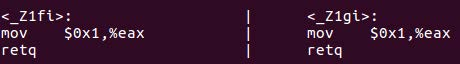
\includegraphics[width=0.9\textwidth]{content/3/chapter10/images/1.jpg}\\
Figure 10.1 – x86 assembly output before (left) and after (right) the aliasing optimization
\end{center}

Figure 10.1 shows the x86 assembly generated by GCC for the increment operations (we omit the function call and the branch, which are identical in both cases). With the aliasing, the compiler has to do two reads from memory (mov instructions). With the manual optimization, there is only one read.

How important are these optimizations? It depends on many factors, so you should not embark on a project to eliminate all aliasing in your code without doing some measurements first. Profiling your code will tell you which parts are performance-critical; there, you have to examine all optimization opportunities. Optimizations that end up helping the compiler by supplying it with additional knowledge are often some of the easiest to implement (the compiler does the hard work). 

The flipside of the recommendation to supply the compiler with hard-to-discover information about your program is this: don't worry about things the compiler can figure out easily. This issue comes up in different contexts, but one of the more common scenarios is using functions that validate their inputs. In your library, you have a swap function that works on pointers:

\begin{lstlisting}[style=styleCXX]
template <typename T>
void my_swap(T* p, T* q) {
	if (p && q) {
		using std::swap;
		swap(*p, *q);
	}
}
\end{lstlisting}

The function accepts null pointers but doesn't do anything with them. In your own code, for some reason, you have to check the pointers anyway, and you call my\_swap() only if both are non-null (maybe you need to do something else if they are null, so you have to check). Ignoring all the other work you may do, the calling code looks like this:

\begin{lstlisting}[style=styleCXX]
void f(int* p, int* q) {
	if (p && q) my_swap(p, q);
}
\end{lstlisting}

An inordinate amount of time is spent by C++ programmers arguing whether the redundant check affects the performance. Should we try to remove the check at the call site? Assuming we cannot, should we create another version of my\_swap() that does not test its inputs? The key observation here is that the function my\_swap() is a template (and a small function), so it is almost certainly going to be inlined. The compiler has all the necessary information to determine that the second test for null is redundant. Does it? Instead of trying to benchmark the possible performance difference (which would be very small in any case), we will compare the assembly output of both programs. If the compiler generates identical machine code with and without the redundant if() statement, we can be certain that there is no performance difference. Here is the assembly output on x86 generated by GCC:

\hspace*{\fill} \\ %插入空行
\begin{center}
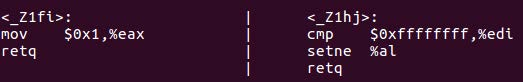
\includegraphics[width=0.9\textwidth]{content/3/chapter10/images/2.jpg}\\
Figure 10.2 – Assembly output with (left) and without (right) redundant pointer test
\end{center}

On the left in Figure 10.2 is the code generated for the program with two if() statements, one inside my\_swap() and one outside. On the right is the code for the program with a special non-testing version of my\_swap(). You can see that the machine code is absolutely identical (if you can read x86 assembly, you will also notice that there are only two comparisons in both cases, not four). 

As we already said, the inlining plays the crucial role here: if my\_swap() wasn't inlined, the first test, in function f(), is good because it avoids the unnecessary function call and allows the compiler to optimize the calling code better for the case when one of the pointers is null. The test inside my\_swap() is now redundant, but the compiler will generate it anyway because it doesn't know whether my\_swap() is called elsewhere, maybe without any guarantees on inputs. It is still highly unlikely that the performance difference would be measurable because the second test is 100\% predictable by the hardware (we talked about this in Chapter 3, CPU Architecture, Resources, and Performance Implications).

By the way, the most common example of this situation is probably the operator delete: C++ allows deleting a null pointer (nothing happens). However, many programmers still write code like this:

\begin{lstlisting}[style=styleCXX]
if (p) delete p; 
\end{lstlisting}

Does it impact the performance, even in theory? No: you can look at the assembly output and convince yourself that, with or without the extra check, there is only one comparison with null. 

Now that you have a better understanding of how the compiler sees your program, let us see one more useful technique for getting better optimization out of the compiler.

\subsubsubsection{10.2.4\hspace{0.2cm}Lifting knowledge from runtime to compile time}

The method we are about to discuss here boils down to one thing: give the compiler more information about the program, in this case, by converting runtime information into compile-time information. In the following example, we need to process a lot of geometric objects represented by the Shape class. They are stored in a container (if the type is polymorphic, it would be a container of pointers). The processing consists of doing one of two operations: we either shrink each object or grow it. Let's see how:

\hspace*{\fill} \\ %插入空行
\noindent
\textbf{06\_template.C}
\begin{lstlisting}[style=styleCXX]
enum op_t { do_shrink, do_grow };
void process(std::vector<Shape>& v, op_t op) {
	for (Shape& s : v) {
		if (op == do_shrink) s.shrink();
		else s.grow();
	}
}
\end{lstlisting}

To generalize, we have a function whose behavior is controlled by one or more configuration variables at runtime. Often, these variables are Boolean (for readability, we chose an enum). We have already seen that if the configuration parameter op is passed by reference, the compiler has to leave the comparison inside the loop and evaluate it for every shape. Even if the parameter is passed by value, many compilers will not hoist the branch out of the loop: it requires duplicating the body of the loop (one loop for shrink and one for grow), and the compilers are wary of bloating the code too much. 

This concern should be taken seriously: a larger executable takes longer to load, and more code increases the stress on the instruction cache (i-cache, used to cache the upcoming instructions the same way as the data caches cache the data that is about to be used by the CPU). However, in some cases, this optimization is still the right choice: often, you know that a lot of data is processed without changing the configuration variables. Maybe these variables are even constant for the entire run of the program (you load the configuration once and use it). 

It is easy to rewrite our simple example to move the branch out of the loop, but if the code is complex, so is the refactoring. We can get some assistance from the compiler if we are willing to give it assistance in turn. The idea is to convert the runtime value into the compile-time one:

\hspace*{\fill} \\ %插入空行
\noindent
\textbf{06\_template.C}
\begin{lstlisting}[style=styleCXX]
template <op_t op>
void process(std::vector<Shape>& v) {
	for (Shape& s : v) {
		if (op == do_shrink) s.shrink();
		else s.grow();
	}
}
void process(std::vector<Shape>& v, op_t op) {
	if (op == do_shrink) process<do_shrink>(v);
	else process<do_grow>(v);
}
\end{lstlisting}

The entire (potentially large) old function process() is converted to a template, but other than that, there are no changes. Specifically, we did not move the branch out of the loop. However, the condition controlling the branch is now a compile-time constant (the template parameter). The compiler will eliminate the branch, and the corresponding dead code, in each template instantiation. In the rest of our program, the configuration variable is still a runtime value, just one that doesn't change very often (or not at all). So we still need a runtime test, but it is used only to decide which template instantiation to call.

This approach can be generalized. Imagine that we need to compute some properties for each shape, like volume, dimensions, weight, and so on. This is all done by a single function because a lot of the calculations are shared between different properties. But it takes time to compute properties we do not need, so we may implement a function like this:

\begin{lstlisting}[style=styleCXX]
void measure(const std::vector<Shape>& s,
	double* length, double* width, double* depth,
	double* volume, double* weight);
\end{lstlisting}

A null pointer is valid and indicates that we do not need that result. Inside the function, we write the code optimally for a particular combination of requested values: we do common computations only once, and we don't compute anything we do not need. However, this check is done inside the loop over shapes, and this time, it is a pretty complex set of conditions. If we need to process a lot of shapes for the same set of measurements, hoisting the conditions out of the loop makes sense, but the compiler is unlikely to do it, even if it can. Again, we can write a template with many non-type parameters: they will be Boolean values like need\_length, need\_width, and so on. Inside that template, the compiler will eliminate all the branches that never get executed for a particular combination of measurements because now this is compile-time information. The function that is called at runtime has to forward the call to the correct template instantiation based on which pointers are non-null. One of the most efficient implementations of this is a lookup table:

\hspace*{\fill} \\ %插入空行
\noindent
\textbf{07\_measure.C}
\begin{lstlisting}[style=styleCXX]
template <bool use_length, bool use_width, …>
void measure(const std::vector<Shape>& v,
double* length, … );
void measure(const std::vector<Shape>& v,
double* length, … ) {
	const int key = ((length != nullptr) << 0) |
					((width  != nullptr) << 1) |
				    ((depth  != nullptr) << 2) |
				    ((volume != nullptr) << 3) |
				    ((weight != nullptr) << 4);
	switch (key) {
		case 0x01: measure<true , false, … >(v, length, … );
		break;
		case 0x02: measure<false, true , … >(v, length, … );
		break;
		…
		default:; // Programming error, assert
	}
}
\end{lstlisting}

This generates a great deal of code: each variant of the measurement is a new function. The effect of such a significant transformation should always be validated by profiling. However, in cases where the measurements are relatively simple (say, many shapes are a cube) and the same set of measurements is requested for many (millions) of shapes, this change can yield substantial performance gains. 

When working with a particular compiler, it pays to know its capabilities, including the optimizations. Such level of detail is beyond the scope of this book, and it is volatile knowledge – the compilers evolve quickly. Instead, this chapter lays the foundation for the understanding of compiler optimizations and gives you, the reader, the frame of reference to advance your understanding. Let us recap the main points of what we learned.


